% Options for packages loaded elsewhere
\PassOptionsToPackage{unicode}{hyperref}
\PassOptionsToPackage{hyphens}{url}
%
\documentclass[
]{book}
\usepackage{amsmath,amssymb}
\usepackage{lmodern}
\usepackage{ifxetex,ifluatex}
\ifnum 0\ifxetex 1\fi\ifluatex 1\fi=0 % if pdftex
  \usepackage[T1]{fontenc}
  \usepackage[utf8]{inputenc}
  \usepackage{textcomp} % provide euro and other symbols
\else % if luatex or xetex
  \usepackage{unicode-math}
  \defaultfontfeatures{Scale=MatchLowercase}
  \defaultfontfeatures[\rmfamily]{Ligatures=TeX,Scale=1}
\fi
% Use upquote if available, for straight quotes in verbatim environments
\IfFileExists{upquote.sty}{\usepackage{upquote}}{}
\IfFileExists{microtype.sty}{% use microtype if available
  \usepackage[]{microtype}
  \UseMicrotypeSet[protrusion]{basicmath} % disable protrusion for tt fonts
}{}
\makeatletter
\@ifundefined{KOMAClassName}{% if non-KOMA class
  \IfFileExists{parskip.sty}{%
    \usepackage{parskip}
  }{% else
    \setlength{\parindent}{0pt}
    \setlength{\parskip}{6pt plus 2pt minus 1pt}}
}{% if KOMA class
  \KOMAoptions{parskip=half}}
\makeatother
\usepackage{xcolor}
\IfFileExists{xurl.sty}{\usepackage{xurl}}{} % add URL line breaks if available
\IfFileExists{bookmark.sty}{\usepackage{bookmark}}{\usepackage{hyperref}}
\hypersetup{
  pdftitle={Visualisering af biologiske datasæt - 2022},
  pdfauthor={Sarah Rennie},
  hidelinks,
  pdfcreator={LaTeX via pandoc}}
\urlstyle{same} % disable monospaced font for URLs
\usepackage{color}
\usepackage{fancyvrb}
\newcommand{\VerbBar}{|}
\newcommand{\VERB}{\Verb[commandchars=\\\{\}]}
\DefineVerbatimEnvironment{Highlighting}{Verbatim}{commandchars=\\\{\}}
% Add ',fontsize=\small' for more characters per line
\usepackage{framed}
\definecolor{shadecolor}{RGB}{248,248,248}
\newenvironment{Shaded}{\begin{snugshade}}{\end{snugshade}}
\newcommand{\AlertTok}[1]{\textcolor[rgb]{0.94,0.16,0.16}{#1}}
\newcommand{\AnnotationTok}[1]{\textcolor[rgb]{0.56,0.35,0.01}{\textbf{\textit{#1}}}}
\newcommand{\AttributeTok}[1]{\textcolor[rgb]{0.77,0.63,0.00}{#1}}
\newcommand{\BaseNTok}[1]{\textcolor[rgb]{0.00,0.00,0.81}{#1}}
\newcommand{\BuiltInTok}[1]{#1}
\newcommand{\CharTok}[1]{\textcolor[rgb]{0.31,0.60,0.02}{#1}}
\newcommand{\CommentTok}[1]{\textcolor[rgb]{0.56,0.35,0.01}{\textit{#1}}}
\newcommand{\CommentVarTok}[1]{\textcolor[rgb]{0.56,0.35,0.01}{\textbf{\textit{#1}}}}
\newcommand{\ConstantTok}[1]{\textcolor[rgb]{0.00,0.00,0.00}{#1}}
\newcommand{\ControlFlowTok}[1]{\textcolor[rgb]{0.13,0.29,0.53}{\textbf{#1}}}
\newcommand{\DataTypeTok}[1]{\textcolor[rgb]{0.13,0.29,0.53}{#1}}
\newcommand{\DecValTok}[1]{\textcolor[rgb]{0.00,0.00,0.81}{#1}}
\newcommand{\DocumentationTok}[1]{\textcolor[rgb]{0.56,0.35,0.01}{\textbf{\textit{#1}}}}
\newcommand{\ErrorTok}[1]{\textcolor[rgb]{0.64,0.00,0.00}{\textbf{#1}}}
\newcommand{\ExtensionTok}[1]{#1}
\newcommand{\FloatTok}[1]{\textcolor[rgb]{0.00,0.00,0.81}{#1}}
\newcommand{\FunctionTok}[1]{\textcolor[rgb]{0.00,0.00,0.00}{#1}}
\newcommand{\ImportTok}[1]{#1}
\newcommand{\InformationTok}[1]{\textcolor[rgb]{0.56,0.35,0.01}{\textbf{\textit{#1}}}}
\newcommand{\KeywordTok}[1]{\textcolor[rgb]{0.13,0.29,0.53}{\textbf{#1}}}
\newcommand{\NormalTok}[1]{#1}
\newcommand{\OperatorTok}[1]{\textcolor[rgb]{0.81,0.36,0.00}{\textbf{#1}}}
\newcommand{\OtherTok}[1]{\textcolor[rgb]{0.56,0.35,0.01}{#1}}
\newcommand{\PreprocessorTok}[1]{\textcolor[rgb]{0.56,0.35,0.01}{\textit{#1}}}
\newcommand{\RegionMarkerTok}[1]{#1}
\newcommand{\SpecialCharTok}[1]{\textcolor[rgb]{0.00,0.00,0.00}{#1}}
\newcommand{\SpecialStringTok}[1]{\textcolor[rgb]{0.31,0.60,0.02}{#1}}
\newcommand{\StringTok}[1]{\textcolor[rgb]{0.31,0.60,0.02}{#1}}
\newcommand{\VariableTok}[1]{\textcolor[rgb]{0.00,0.00,0.00}{#1}}
\newcommand{\VerbatimStringTok}[1]{\textcolor[rgb]{0.31,0.60,0.02}{#1}}
\newcommand{\WarningTok}[1]{\textcolor[rgb]{0.56,0.35,0.01}{\textbf{\textit{#1}}}}
\usepackage{longtable,booktabs,array}
\usepackage{calc} % for calculating minipage widths
% Correct order of tables after \paragraph or \subparagraph
\usepackage{etoolbox}
\makeatletter
\patchcmd\longtable{\par}{\if@noskipsec\mbox{}\fi\par}{}{}
\makeatother
% Allow footnotes in longtable head/foot
\IfFileExists{footnotehyper.sty}{\usepackage{footnotehyper}}{\usepackage{footnote}}
\makesavenoteenv{longtable}
\usepackage{graphicx}
\makeatletter
\def\maxwidth{\ifdim\Gin@nat@width>\linewidth\linewidth\else\Gin@nat@width\fi}
\def\maxheight{\ifdim\Gin@nat@height>\textheight\textheight\else\Gin@nat@height\fi}
\makeatother
% Scale images if necessary, so that they will not overflow the page
% margins by default, and it is still possible to overwrite the defaults
% using explicit options in \includegraphics[width, height, ...]{}
\setkeys{Gin}{width=\maxwidth,height=\maxheight,keepaspectratio}
% Set default figure placement to htbp
\makeatletter
\def\fps@figure{htbp}
\makeatother
\setlength{\emergencystretch}{3em} % prevent overfull lines
\providecommand{\tightlist}{%
  \setlength{\itemsep}{0pt}\setlength{\parskip}{0pt}}
\setcounter{secnumdepth}{5}
\usepackage{booktabs}
\ifluatex
  \usepackage{selnolig}  % disable illegal ligatures
\fi
\usepackage[]{natbib}
\bibliographystyle{apalike}

\title{Visualisering af biologiske datasæt - 2022}
\author{Sarah Rennie}
\date{Last updated: 2022-04-21}

\begin{document}
\maketitle

{
\setcounter{tocdepth}{1}
\tableofcontents
}
\hypertarget{basics}{%
\chapter{Grundlæggende R}\label{basics}}

\hypertarget{inledning-til-kapitel}{%
\section{Inledning til kapitel}\label{inledning-til-kapitel}}

Her opsummerer jeg nogle grundlæggende R og statistik, der betragtes som forudsætninger i det nuværende kursus. Selvom vi i kurset skifter hurtigt over til den tidyverse-pakke løsning, som erstatter meget af funktionaliteten fra base-R, er det stadig vigtigt at have et grundlæggende kendskab til hvordan tingene fungerer i base-R - derfor hvis du har meget lidt erfaring med base-R anbefaler jeg, at du også bruger noget ekstra tid udover den første mødegange til at komme op på niveauet.

For at bestå kurset er det ikke forventningen, at du kender til alle detaljer og teori bag de statistiske metoder, men at du kan anvende dem hensigtsmæssigt i praksis i R, samt fortolke resultaterne. Jeg giver masser af muligheder for at øve dig med at lave statistik hele vejen gennem kurset, og i selve eksamen stiller jeg ikke spørgsmål om metoder, der ikke bliver dækkede blandt de forskellige øvelser (herunder workshop opgaver). Jeg kommer også ind på lineær regression igen senere gennem forelæsningerne så vær ikke bekymret hvis du ikke har set det hele før.

Se gerne også ``Quiz - grundlæggende'' på Absalon for at tjekke din forståelse og udfylde eventuelle huller i din viden (OBS: Quizzen er tilgængelig lidt inden starten af kurset).

\hypertarget{rstudio}{%
\section{RStudio}\label{rstudio}}

Vi kommer fremadrettet til at være afhængig af RStudio til at lave blandt andet R Markdown dokumenter. Kendskab til R Markdown er emnet i vores næste lektion og jeg antager, at du ikke har benyttet det før.

Det allerførste du skulle gør, hvis du ikke har installeret RStudio på din computer, er at downloade det gratis på nettet:

\url{https://www.rstudio.com/products/rstudio/download/\#download}

Følg venligst RStudios egne anvisninger til at få det installeret. Bemærk, at installering af RStudio er ikke den samme som at have R installeret på din computer - man skal installere dem begge to (man kan bruge R uden RStudio men ikke omvendt.

\hypertarget{de-forskellige-vinduer-i-rstudio}{%
\subsection{De forskellige vinduer i RStudio}\label{de-forskellige-vinduer-i-rstudio}}

Du kan læse følgende for at lære de fire forskellige vinduer i RStudio at kende:

\url{https://bookdown.org/ndphillips/YaRrr/the-four-rstudio-windows.html}

Her er et kort oversigt:

\begin{itemize}
\tightlist
\item
  Man skriver kode i \textbf{Source} (øverst til venstre)
\item
  Man kører kode ved at tryk CMD+ENTER (eller WIN-KEY+ENTER)
\item
  Koder køres ind i \textbf{Console} (som plejer at være nederst til venstre, selvom det er øverst til højere i billedet). Man kan også skrive koder direkte i Console, men det ikke anbefales generelt, når koden ikke bliver gemt.
\item
  \textbf{Environment} - her kan man se blandt andet, alle objekter i Workspace.
\end{itemize}

\hypertarget{working-directory}{%
\section{Working directory}\label{working-directory}}

Når man arbejder på et projekt, er det ofte nyttigt at vide, den \emph{working directory} som R arbejder fra - det er den mappe, hvor R forsøger at åbne eller gemme filer fra, medmindre man angiver et andet sted.

\begin{Shaded}
\begin{Highlighting}[]
\FunctionTok{getwd}\NormalTok{() }\CommentTok{\#se nuværende working directory}
\FunctionTok{list.dirs}\NormalTok{(}\AttributeTok{path =} \StringTok{"."}\NormalTok{, }\AttributeTok{recursive =} \ConstantTok{FALSE}\NormalTok{) }\CommentTok{\#se mappe indenfor working directory}
\FunctionTok{setwd}\NormalTok{(}\StringTok{"\textasciitilde{}/Documents/"}\NormalTok{) }\CommentTok{\#sætte en ny working directory (C:/Users/myname/Documents hvis man bruger Windows)}
\end{Highlighting}
\end{Shaded}

Hvis man bruger Windows, husk at man kan skrive en path på følgende måde:

\begin{Shaded}
\begin{Highlighting}[]
\CommentTok{\#notrun}
\FunctionTok{setwd}\NormalTok{(}\StringTok{"C:/Users/myname/Documents"}\NormalTok{) }\CommentTok{\#enten med /}
\FunctionTok{setwd}\NormalTok{(}\StringTok{"C:}\SpecialCharTok{\textbackslash{}\textbackslash{}}\StringTok{Users}\SpecialCharTok{\textbackslash{}\textbackslash{}}\StringTok{myname}\SpecialCharTok{\textbackslash{}\textbackslash{}}\StringTok{Documents"}\NormalTok{) }\CommentTok{\#eller med \textbackslash{}\textbackslash{}}
\end{Highlighting}
\end{Shaded}

\textbf{OBS}: jeg bruger Mac, så hvis der er et vigtigt ting at man skal huske hvis man bruger en Windows computer, kan jeg også tilføje det her. Bemærk dog, at de allerfleste ting ved R programmering og tidyverse er ens uanset om man bruger Windows eller Mac.

\hypertarget{r-pakker}{%
\section{R pakker}\label{r-pakker}}

R pakker er simpelthen en samling af funktioner (eller datasæt i nogle tilfælde), der udvider hvad er tilgængelige i base-R (den R man få, uden at indlæse en pakke). I R er der mange tusind R pakker (op mod 100,000), der er tilgængelige på \textbf{CRAN} (\url{https://cran.r-project.org/}). Indenfor det biologiske fag er der også mange flere pakker på \textbf{Bioconductor} (\url{https://www.bioconductor.org/}), og i nogle tilfælde kan R pakker også installeres direkte fra \textbf{Github}.

I dette kursus arbejder vi rigtig meget med en pakke der hedder \textbf{tidyverse}. \textbf{tidyverse} er faktisk en samling af otte R pakker, som indlæses på en gang. Inden du indlæse pakken, skal du først sikre dig, at pakken er installeret på systemet ved følgende kommando:

\begin{Shaded}
\begin{Highlighting}[]
\FunctionTok{install.packages}\NormalTok{(}\StringTok{"tidyverse"}\NormalTok{)}
\end{Highlighting}
\end{Shaded}

Alle pakker på \textbf{CRAN} er installeret på samme måde. Når du faktisk gerne vil bruge en R pakke, skal du først indlæse den ved at bruge \texttt{library()}:

\begin{Shaded}
\begin{Highlighting}[]
\FunctionTok{library}\NormalTok{(tidyverse)}
\end{Highlighting}
\end{Shaded}

\begin{verbatim}
## -- Attaching packages --------------------------------------- tidyverse 1.3.1 --
\end{verbatim}

\begin{verbatim}
## v ggplot2 3.3.5     v purrr   0.3.4
## v tibble  3.1.6     v dplyr   1.0.8
## v tidyr   1.2.0     v stringr 1.4.0
## v readr   2.1.2     v forcats 0.5.1
\end{verbatim}

\begin{verbatim}
## -- Conflicts ------------------------------------------ tidyverse_conflicts() --
## x dplyr::filter() masks stats::filter()
## x dplyr::lag()    masks stats::lag()
\end{verbatim}

Vi kommer til at arbejde med \textbf{tidyverse} pakker fra kapitel tre (vi starter med \textbf{ggplot2} og så nogle af de andre pakke fra \textbf{tidyverse} fra kapitel fire), \textbf{så det er en god idé at har tidyverse installeret allerede nu}, når det nogle gange kan tage lidt tid til at installere eller opdatere de mange andre mulige pakker, der \textbf{tidyverse} er afhængig af.

Vær opmærksom på, at der nogle gange opstår konflikter når det samme funktionnavn findes i flere pakker - for eksempel, funktionen \texttt{filter()} findes indenfor to forskellige pakker, nemlig \texttt{dplyr} og \texttt{stats}. Når du skriver \texttt{filter()} så ved R ikke, hvilke pakker du mener. I dette tilfælde kan du være gennemskueligt overfor den pakke, du gerne vil bruge ved at skrive \texttt{dplyr::filter()} eller \texttt{stats:filter()} i stedet for bare \texttt{filter()}.

Som sidste kommentar, er det god praksis at indlæse alle pakker, der du benytter sig af, på toppen af din script, så at du hurtigt kan få overblik over, hvilke pakker, der skal indlæses til at få dine koder til at fungere.

\hypertarget{hvor-kommer-vores-data-fra}{%
\section{Hvor kommer vores data fra?}\label{hvor-kommer-vores-data-fra}}

De forskellige datasæt, vi kommer til at arbejde med i kurset stammer fra mange forskellige steder.

\hypertarget{indbyggede-datasuxe6t}{%
\subsection{Indbyggede datasæt}\label{indbyggede-datasuxe6t}}

I R er der mange indbygget datasæt som er meget brugbart for at vise koncepter, hvilket gøre dem især populært i undervisningsmateriale. Indbyggede datasæt er ofte tilgængligt indenfor mange pakker, men \texttt{library(datasets)} er den mest brugt (der er også mange indenfor \texttt{library(ggplot2)}. For eksempel, for at indlæse datasættet, der hedder `iris', kan man bruge \texttt{data()}:

\begin{Shaded}
\begin{Highlighting}[]
\FunctionTok{library}\NormalTok{(datasets)}
\FunctionTok{data}\NormalTok{(iris)}
\end{Highlighting}
\end{Shaded}

Så er en \emph{dataframe}, der hedder `iris' tilgængelige som en \emph{objekt} i \emph{workspacen} - se den ``Environment'' fane på højere side i RStudio, eller indtaste \texttt{ls()}, så bør du kunne se et objekt med navnet `iris'. Man kan kun arbejde med objekter som er en del af workspacen.

\hypertarget{importering-af-data-fra-.txt-fil}{%
\subsection{Importering af data fra .txt fil}\label{importering-af-data-fra-.txt-fil}}

Det er meget hyppigt, at man har sin data i formen af en .txt fil eller .xlsx fil på sin computer. Den nemmeste måde at få åbnet en .txt fil er ved at bruge \texttt{read.table()}, som i nedenstående:

\begin{Shaded}
\begin{Highlighting}[]
\NormalTok{data }\OtherTok{\textless{}{-}} \FunctionTok{read.table}\NormalTok{(}\StringTok{"mydata.txt"}\NormalTok{) }\CommentTok{\#indlæse data filen mydata.txt som er i working directory}
\FunctionTok{head}\NormalTok{(data)}
\end{Highlighting}
\end{Shaded}

Hvis datasættet har kolonner navne, der er skrevet ind i filen, så skal man huske at bruge \texttt{header=T} for at undgå, at den første række i datasættet bliver disse tekste i stedet for virkelige observationer.

\begin{Shaded}
\begin{Highlighting}[]
\NormalTok{data }\OtherTok{\textless{}{-}} \FunctionTok{read.table}\NormalTok{(}\StringTok{"mydata.txt"}\NormalTok{,}\AttributeTok{header=}\NormalTok{T) }\CommentTok{\#indlæse data filen mydata.txt som er i working directory}
\FunctionTok{head}\NormalTok{(data)}
\end{Highlighting}
\end{Shaded}

\hypertarget{importering-af-data-fra-excel}{%
\subsection{Importering af data fra Excel}\label{importering-af-data-fra-excel}}

Der findes også en hjælpsom pakke, som hedder \textbf{readxl}, der kan indlæse Excel-ark direkte ind i R:

\begin{Shaded}
\begin{Highlighting}[]
\FunctionTok{library}\NormalTok{(readxl)}
\NormalTok{data }\OtherTok{\textless{}{-}} \FunctionTok{read\_excel}\NormalTok{(}\StringTok{"data.xlsx"}\NormalTok{)}
\NormalTok{data}
\end{Highlighting}
\end{Shaded}

\hypertarget{kaggle}{%
\subsection{Kaggle}\label{kaggle}}

Hvis du gerne vil øve dig med statistike analyser (udover nuværende kursus), er Kaggle en fantastisk ressource til at finde forskellige datasæt. I rigtige mange tilfælde kan man også finde analyser some andre har lavet I R (også Python), hvilket kan inspirere jeres egen læring.

Link hvis interesseret: \url{https://www.kaggle.com/}

\hypertarget{beregninger-i-r}{%
\section{Beregninger i R}\label{beregninger-i-r}}

Her er nogle helt grundlæggende koncepter når man arbejder med R. Du må selvfølgelige gerne springe sektionen over, hvis du allerede har meget erfaring med base R, men det kan være værd at tjekke, om der noget ting, der lige skal gennemgås. En god tilgang er bare at arbejde gennem problemstillingerne nedenfor, og bruger følgende notater som en reference.

\hypertarget{vectorer}{%
\subsection{Vectorer}\label{vectorer}}

I R laver man en vector med \texttt{c()}, hvor man adskiller de forskellige elementer med en komma, som i nedenstående eksempel:

\begin{Shaded}
\begin{Highlighting}[]
\NormalTok{a }\OtherTok{\textless{}{-}} \FunctionTok{c}\NormalTok{(}\DecValTok{1}\NormalTok{,}\DecValTok{2}\NormalTok{,}\DecValTok{3}\NormalTok{,}\DecValTok{4}\NormalTok{,}\DecValTok{5}\NormalTok{) }\CommentTok{\#sæt objektet \textquotesingle{}a\textquotesingle{} til at være en vector af tal }
\NormalTok{a}
\end{Highlighting}
\end{Shaded}

\begin{verbatim}
## [1] 1 2 3 4 5
\end{verbatim}

Man er ikke begrænset til tal:

\begin{Shaded}
\begin{Highlighting}[]
\NormalTok{c }\OtherTok{\textless{}{-}} \FunctionTok{c}\NormalTok{(}\StringTok{"cat"}\NormalTok{,}\StringTok{"mouse"}\NormalTok{,}\StringTok{"horse"}\NormalTok{,}\StringTok{"sheep"}\NormalTok{,}\StringTok{"dog"}\NormalTok{)}
\NormalTok{c}
\end{Highlighting}
\end{Shaded}

\begin{verbatim}
## [1] "cat"   "mouse" "horse" "sheep" "dog"
\end{verbatim}

\hypertarget{datatyper}{%
\subsection{datatyper}\label{datatyper}}

Nar vi kommer til at arbejde med visualiseringer og data beardejdning er det vigtigt at have styr på datatyper i datasættet. For eksempel har vectoren \texttt{c} ovenpå typen \texttt{character} (forkortet \texttt{chr}) og ikke \texttt{numeric} (forkortet \texttt{num}):

\begin{Shaded}
\begin{Highlighting}[]
\FunctionTok{is.numeric}\NormalTok{(c)}
\DocumentationTok{\#\# [1] FALSE}
\FunctionTok{is.character}\NormalTok{(c)}
\DocumentationTok{\#\# [1] TRUE}
\end{Highlighting}
\end{Shaded}

Her er en list overfor nogle af de vigtigste datatyper:

\begin{longtable}[]{@{}
  >{\raggedright\arraybackslash}p{(\columnwidth - 4\tabcolsep) * \real{0.33}}
  >{\raggedright\arraybackslash}p{(\columnwidth - 4\tabcolsep) * \real{0.42}}
  >{\raggedright\arraybackslash}p{(\columnwidth - 4\tabcolsep) * \real{0.25}}@{}}
\toprule
Datatype & Navn & Beskrivelse \\
\midrule
\endhead
\texttt{int} & integer & kun hel tal \texttt{c(-1,0,1,2,3)} \\
\texttt{lgl} & logical & \texttt{TRUE\ TRUE\ FALSE\ TRUE\ FALSE} \\
\texttt{chr} & character & \texttt{c("Bob","Sally","Brian",...)} \\
\texttt{fct} & factor & bestemte niveauer e.g.~\texttt{Species}: \texttt{c("setosa","versicola")} \\
\texttt{dbl} & double & Tal fk. c(\texttt{4.3902}, \texttt{3.12}, \texttt{4.5}) \\
\texttt{lst} & list & blande forskellige data typer og specificere elementer med \texttt{{[}{[}i{]}{]}} \texttt{{[}{[}1{]}{]}\ {[}1{]}\ c("red","blue")} \texttt{{[}{[}2{]}{]}\ {[}1{]}\ TRUE} \texttt{{[}{[}3{]}{]}\ {[}1{]}\ c(3,2.3,1.459)} \\
\bottomrule
\end{longtable}

En datatype, der bør få særlig opmærksomhed er \texttt{fct} (factor). I følgende vector \texttt{tea\_coffee} har vi tekst, men blandt de fem elementer er der kun to bestemte niveauer (nemlig ``tea'' og ``coffee'').

\begin{Shaded}
\begin{Highlighting}[]
\NormalTok{tea\_coffee }\OtherTok{\textless{}{-}} \FunctionTok{c}\NormalTok{(}\StringTok{"tea"}\NormalTok{,}\StringTok{"tea"}\NormalTok{,}\StringTok{"coffee"}\NormalTok{,}\StringTok{"coffee"}\NormalTok{,}\StringTok{"tea"}\NormalTok{)}
\FunctionTok{is.factor}\NormalTok{(tea\_coffee)}
\DocumentationTok{\#\# [1] FALSE}
\NormalTok{tea\_coffee}
\DocumentationTok{\#\# [1] "tea"    "tea"    "coffee" "coffee" "tea"}
\end{Highlighting}
\end{Shaded}

Vi vil derfor gerne fortælle R, at \texttt{tea\_coffee} er ikke bare nogle tilfældig tekst men at der er en struktur med, så vi bruger funktionen \texttt{as.factor} for at lave den om til datatypen \texttt{fct}.

\begin{Shaded}
\begin{Highlighting}[]
\NormalTok{tea\_coffee }\OtherTok{\textless{}{-}} \FunctionTok{as.factor}\NormalTok{(tea\_coffee)}
\FunctionTok{is.factor}\NormalTok{(tea\_coffee)}
\DocumentationTok{\#\# [1] TRUE}
\NormalTok{tea\_coffee}
\DocumentationTok{\#\# [1] tea    tea    coffee coffee tea   }
\DocumentationTok{\#\# Levels: coffee tea}
\end{Highlighting}
\end{Shaded}

Den `ekstra' oplysninger man har ved at sige, at en variabel betragtes som factor bliver vigtigt når man arbejder med visualiseringer - for eksempel, hvis vi gerne vil lave et barplot hvor man gerne vil adskille søjlerne efter de to niveauer ``tea'' og ``coffee'' (visualiseringer er emnet fra kapitel 3).

\hypertarget{dataframes}{%
\section{Dataframes}\label{dataframes}}

\url{http://www.r-tutor.com/r-introduction/data-frame}

Mange af de ting, som vi laver i R tager udgangspunkten i dataframes (eller datarammer).

\begin{Shaded}
\begin{Highlighting}[]
\NormalTok{mydf }\OtherTok{\textless{}{-}} \FunctionTok{data.frame}\NormalTok{(}\StringTok{"personID"}\OtherTok{=}\DecValTok{1}\SpecialCharTok{:}\DecValTok{5}\NormalTok{, }\StringTok{"height"}\OtherTok{=}\FunctionTok{c}\NormalTok{(}\DecValTok{140}\NormalTok{,}\DecValTok{187}\NormalTok{,}\DecValTok{154}\NormalTok{,}\DecValTok{132}\NormalTok{,}\DecValTok{165}\NormalTok{), }\StringTok{"age"}\OtherTok{=}\FunctionTok{c}\NormalTok{(}\DecValTok{34}\NormalTok{,}\DecValTok{31}\NormalTok{,}\DecValTok{25}\NormalTok{,}\DecValTok{43}\NormalTok{,}\DecValTok{29}\NormalTok{))}
\NormalTok{mydf}
\end{Highlighting}
\end{Shaded}

\begin{verbatim}
##   personID height age
## 1        1    140  34
## 2        2    187  31
## 3        3    154  25
## 4        4    132  43
## 5        5    165  29
\end{verbatim}

Man kan fa adgang til variabler i en dataframe ved at bruge det dollar tegn \texttt{\$}. For eksempel giver følgende variablen \texttt{personID} fra dataframen \texttt{mydf}:

\begin{Shaded}
\begin{Highlighting}[]
\NormalTok{mydf}\SpecialCharTok{$}\NormalTok{personID}
\end{Highlighting}
\end{Shaded}

\begin{verbatim}
## [1] 1 2 3 4 5
\end{verbatim}

Husk, at vores dataframe, ligesom et matrix (i R: \texttt{matrix()}) har to dimensioner - række og kolonner Forskellen mellem en matrix og en dataramme er, at datarammer kan indeholde mange forskellige data typer (herunder numeriske, faktorer, karakterer osv.), men matrix indeholder kun numeriske data. For eksempel i tilfældet af ovenstående dataframen er alle variabler numeriske, men vi kan godt tilføje en variabel som er ikke-numeriske:

\begin{Shaded}
\begin{Highlighting}[]
\NormalTok{mydf}\SpecialCharTok{$}\NormalTok{colour }\OtherTok{\textless{}{-}} \FunctionTok{c}\NormalTok{(}\StringTok{"red"}\NormalTok{,}\StringTok{"blue"}\NormalTok{,}\StringTok{"green"}\NormalTok{,}\StringTok{"orange"}\NormalTok{,}\StringTok{"purple"}\NormalTok{) }\CommentTok{\#make new variable which is non{-}numeric}
\NormalTok{mydf}
\end{Highlighting}
\end{Shaded}

\begin{verbatim}
##   personID height age colour
## 1        1    140  34    red
## 2        2    187  31   blue
## 3        3    154  25  green
## 4        4    132  43 orange
## 5        5    165  29 purple
\end{verbatim}

Nu er \texttt{mydf} er en dataframe, der blander forskellige datatyper, men følgende er en matrix

\begin{Shaded}
\begin{Highlighting}[]
\FunctionTok{matrix}\NormalTok{(}\FunctionTok{c}\NormalTok{(}\DecValTok{1}\NormalTok{, }\DecValTok{2}\NormalTok{, }\DecValTok{3}\NormalTok{, }\DecValTok{4}\NormalTok{, }\DecValTok{5}\NormalTok{, }\DecValTok{6}\NormalTok{), }
    \AttributeTok{nrow=}\DecValTok{3}\NormalTok{,}
    \AttributeTok{ncol=}\DecValTok{2}\NormalTok{)}
\end{Highlighting}
\end{Shaded}

\begin{verbatim}
##      [,1] [,2]
## [1,]    1    4
## [2,]    2    5
## [3,]    3    6
\end{verbatim}

og kan kun indeholde numeriske data, som kan bruges til at lave matematik operationer (matrix multiplikation osv.). I dette kursus beskæftiger os primært med dataframes (som bliver kaldt for tibbles i \textbf{tidyverse}).

\hypertarget{delmuxe6gder-af-dataframes}{%
\subsection{Delmægder af dataframes}\label{delmuxe6gder-af-dataframes}}

Selvom vi kommer til at redefinere hvordan man laver delmængde når vi kommer til at arbejde med pakken \textbf{tidyverse}, er det alligevel vigtigt at forstå, hvordan man laver en delmængde i base-R, og det er et område, der ofte skaber forvirring blandt de uerfarne.

Når man vil gerne har en bestemt delmængde af en vector, bruger man firkantet paranteser \texttt{{[}\ {]}}. Følgende kode giver mig de første to værdier fra vectoren \texttt{a}:

\begin{Shaded}
\begin{Highlighting}[]
\NormalTok{a[}\DecValTok{1}\SpecialCharTok{:}\DecValTok{2}\NormalTok{]}
\end{Highlighting}
\end{Shaded}

\begin{verbatim}
## [1] 1 2
\end{verbatim}

Bemærk, at mens vectorer har kun en dimension, \textbf{har dataframes to dimensioner}. Når man skal lave en delmægde af en dataframe, skal man derfor fortælle R, hvilke række og hvilke kolonner skal være med.

\begin{Shaded}
\begin{Highlighting}[]
\NormalTok{mydf[række indekser, kolonner indekser]  }\CommentTok{\#not run}
\end{Highlighting}
\end{Shaded}

For eksempel, hvis vi gerne vil have den første to observationer med, samt kun den anden variabel, skriver man følgende:

\begin{Shaded}
\begin{Highlighting}[]
\NormalTok{mydf[}\DecValTok{1}\SpecialCharTok{:}\DecValTok{2}\NormalTok{, }\DecValTok{2}\NormalTok{]  }\CommentTok{\#first two rows (observations), second column (variable) only}
\end{Highlighting}
\end{Shaded}

\begin{verbatim}
## [1] 140 187
\end{verbatim}

Hvis vi vil beholde den første to observationer og samtlige variabler, kan den anden plads være tom:

\begin{Shaded}
\begin{Highlighting}[]
\NormalTok{mydf[}\DecValTok{1}\SpecialCharTok{:}\DecValTok{2}\NormalTok{, ]  }\CommentTok{\#first two rows, all columns}
\end{Highlighting}
\end{Shaded}

\begin{verbatim}
##   personID height age colour
## 1        1    140  34    red
## 2        2    187  31   blue
\end{verbatim}

Jeg kan også angive et variabelnavn direkte:

\begin{Shaded}
\begin{Highlighting}[]
\NormalTok{mydf[}\DecValTok{1}\SpecialCharTok{:}\DecValTok{2}\NormalTok{,}\StringTok{"height"}\NormalTok{]}
\end{Highlighting}
\end{Shaded}

\begin{verbatim}
## [1] 140 187
\end{verbatim}

Man kan kigge på en subset af rækkerne i de data ved at

\begin{Shaded}
\begin{Highlighting}[]
\NormalTok{mydf[mydf}\SpecialCharTok{$}\NormalTok{height}\SpecialCharTok{\textgreater{}=}\DecValTok{165}\NormalTok{,] }\CommentTok{\#alle rækker i datarammen med height = 165 eller over}
\end{Highlighting}
\end{Shaded}

\begin{verbatim}
##   personID height age colour
## 2        2    187  31   blue
## 5        5    165  29 purple
\end{verbatim}

Her er en tabel af comparitiver, og jeg gengiver samme tabel når I kommer til at lave delmængde i \textbf{tidyverse}:

\begin{longtable}[]{@{}ll@{}}
\toprule
comparitiv & beskrivelse \\
\midrule
\endhead
\texttt{\textless{}} & less than \\
\texttt{\textgreater{}} & greater than \\
\texttt{\textless{}=} & less than or equal to \\
\texttt{\textgreater{}=} & greater than or equal to \\
\texttt{==} & equal to \\
\texttt{!=} & not equal to \\
\texttt{\&} & and \\
\texttt{\%in\%} & in \\
\texttt{\textbar{}} & or \\
\texttt{!} & not \\
\bottomrule
\end{longtable}

Jeg mener, at \texttt{\%in\%} er særlig brugbart og er værd at lære:

\begin{Shaded}
\begin{Highlighting}[]
\NormalTok{mydf[mydf}\SpecialCharTok{$}\NormalTok{personID }\SpecialCharTok{\%in\%} \FunctionTok{c}\NormalTok{(}\DecValTok{1}\NormalTok{,}\DecValTok{3}\NormalTok{,}\DecValTok{5}\NormalTok{),] }\CommentTok{\#alle personer med personID 1,3 eller 5 }
\end{Highlighting}
\end{Shaded}

\begin{verbatim}
##   personID height age colour
## 1        1    140  34    red
## 3        3    154  25  green
## 5        5    165  29 purple
\end{verbatim}

Her er et eksempel på, hvordan man bruger udråbstegnet: personer med personID, der ikke er 1,3 eller 5:

\begin{Shaded}
\begin{Highlighting}[]
\NormalTok{mydf[}\SpecialCharTok{!}\NormalTok{(mydf}\SpecialCharTok{$}\NormalTok{personID }\SpecialCharTok{\%in\%} \FunctionTok{c}\NormalTok{(}\DecValTok{1}\NormalTok{,}\DecValTok{3}\NormalTok{,}\DecValTok{5}\NormalTok{)),] }\CommentTok{\#alle personer med personID 2 eller 4}
\end{Highlighting}
\end{Shaded}

\begin{verbatim}
##   personID height age colour
## 2        2    187  31   blue
## 4        4    132  43 orange
\end{verbatim}

\hypertarget{descriptive-statistics}{%
\section{Descriptive statistics}\label{descriptive-statistics}}

\hypertarget{simulere-data-fra-den-normale-fordeling}{%
\subsection{Simulere data fra den normale fordeling}\label{simulere-data-fra-den-normale-fordeling}}

Hvis du har bruge for at vide mere om den normale fordeling: \url{http://www.r-tutor.com/elementary-statistics/probability-distributions/normal-distribution}

Man kan nemt lave sin egne `fake' data ved at simulere det fra en fordeling, der vil typiske være den normale fordeling, idet den normale fordeling opstår mest hyppigt i den virkelige verden (husk den klassiske klokke-form). I R kan man bruge funktionen \texttt{rnorm} til at simulere data - først angiver man, hvor mange observationer man vil have, og dernæst den mean og standard deviation (sd), som er de to nødvendige parametre for at beskrive en normal fordeling

\begin{Shaded}
\begin{Highlighting}[]
\NormalTok{x }\OtherTok{\textless{}{-}} \FunctionTok{rnorm}\NormalTok{(}\DecValTok{25}\NormalTok{,}\AttributeTok{mean=}\DecValTok{0}\NormalTok{,}\AttributeTok{sd=}\DecValTok{1}\NormalTok{) }\CommentTok{\#standard normal distribution}
\NormalTok{x }\CommentTok{\#så har vi 25 værdier fra en normal distribution med mean=0 og standard deviation=1.}
\end{Highlighting}
\end{Shaded}

\begin{verbatim}
##  [1]  1.4311609704  0.8018335250 -0.7716697451  0.8582603190 -0.3412557958
##  [6]  0.3145008312  0.8988635544  1.2667383590 -0.3310681421  1.4875715490
## [11] -0.6218384931  0.8933896456  1.6796713475  0.1453959907 -0.9608929364
## [16] -0.0009451856 -0.1975433155  1.0002760152  0.4799559210  0.3207776943
## [21] -0.3723581172  0.9618425415 -1.6519491309  0.3935887395 -0.1265245106
\end{verbatim}

I stedet for at kigge på alle værdier på én gang, vil vi måske hellere kigge kun på de første (eller sidste) værdier:

\begin{Shaded}
\begin{Highlighting}[]
\FunctionTok{head}\NormalTok{(x) }\CommentTok{\#første 6}
\DocumentationTok{\#\# [1]  1.4311610  0.8018335 {-}0.7716697  0.8582603 {-}0.3412558  0.3145008}
\FunctionTok{tail}\NormalTok{(x) }\CommentTok{\#sidste 6}
\DocumentationTok{\#\# [1]  0.3207777 {-}0.3723581  0.9618425 {-}1.6519491  0.3935887 {-}0.1265245}
\NormalTok{x[}\DecValTok{1}\NormalTok{] }\CommentTok{\#første værdi}
\DocumentationTok{\#\# [1] 1.431161}
\NormalTok{x[}\FunctionTok{length}\NormalTok{(x)] }\CommentTok{\#sidste data point}
\DocumentationTok{\#\# [1] {-}0.1265245}
\end{Highlighting}
\end{Shaded}

Bemærk, at til forskellen af Python og mange andre programmering sprog, R bruger 1-baserende indicer - det betyder, at den første værdi er \texttt{x{[}1{]}} og \textbf{ikke} \texttt{x{[}0{]}} som i Python.

\hypertarget{measures-of-central-tendency}{%
\subsection{Measures of central tendency}\label{measures-of-central-tendency}}

\begin{longtable}[]{@{}ll@{}}
\toprule
function & Description \\
\midrule
\endhead
\texttt{mean()} & mean \(\bar{x}_{i} = \frac{1}{n}\sum_{i=1}^{n} x_{i}\) \\
\texttt{median()} & median value \\
\texttt{max()} & maximum value \\
\texttt{min()} & minimum value \\
\texttt{var()} & variance \(s^2 = \frac{1}{n-1}\sum_{i=1}^{n} (x_{i} - \bar{x}_{i})^2\) \\
\texttt{sd()} & standard deviation \(s\) \\
\bottomrule
\end{longtable}

Lad os afprøve dem på vores simulerede data:

\begin{Shaded}
\begin{Highlighting}[]
\NormalTok{my\_mean }\OtherTok{\textless{}{-}} \FunctionTok{mean}\NormalTok{(x)}
\NormalTok{my\_median }\OtherTok{\textless{}{-}} \FunctionTok{median}\NormalTok{(x)}
\NormalTok{my\_max }\OtherTok{\textless{}{-}} \FunctionTok{max}\NormalTok{(x)}
\NormalTok{my\_min }\OtherTok{\textless{}{-}} \FunctionTok{min}\NormalTok{(x)}
\NormalTok{my\_var }\OtherTok{\textless{}{-}} \FunctionTok{var}\NormalTok{(x)}
\NormalTok{my\_sd }\OtherTok{\textless{}{-}} \FunctionTok{sd}\NormalTok{(x)}
\FunctionTok{c}\NormalTok{(my\_mean,my\_median,my\_max,my\_min,my\_var,my\_sd) }\CommentTok{\#print results}
\end{Highlighting}
\end{Shaded}

\begin{verbatim}
## [1]  0.3023113  0.3207777  1.6796713 -1.6519491  0.7073302  0.8410292
\end{verbatim}

Man kan også lave et summary af dataen, som bestå af mange af de statistiker navnt ovenpå:

\begin{Shaded}
\begin{Highlighting}[]
\FunctionTok{summary}\NormalTok{(x)}
\end{Highlighting}
\end{Shaded}

\begin{verbatim}
##    Min. 1st Qu.  Median    Mean 3rd Qu.    Max. 
## -1.6519 -0.3311  0.3208  0.3023  0.8989  1.6797
\end{verbatim}

\hypertarget{tapply}{%
\subsection{\texorpdfstring{\texttt{tapply()}}{tapply()}}\label{tapply}}

En meget brugbar funktion, som er værd at vide, er \texttt{tapply()}.

\begin{Shaded}
\begin{Highlighting}[]
\FunctionTok{data}\NormalTok{(iris)}
\FunctionTok{tapply}\NormalTok{(iris}\SpecialCharTok{$}\NormalTok{Sepal.Length,iris}\SpecialCharTok{$}\NormalTok{Species,mean) }\CommentTok{\# ovenstående i kun en linje}
\end{Highlighting}
\end{Shaded}

\begin{verbatim}
##     setosa versicolor  virginica 
##      5.006      5.936      6.588
\end{verbatim}

Her tager vi en variabel der hedder \texttt{Sepal.Length}, opdeler den efter \texttt{Species}, og beregner \texttt{mean} for enhver af de tre arter i \texttt{Species} (setosa, versicolor og virginica). Man kan opnå det samme resultat ved at beregne \texttt{mean} for de tre \texttt{Species} hver for sig (en tilgang, der ikke opskaleres særlig godt!):

\begin{Shaded}
\begin{Highlighting}[]
\CommentTok{\# gennemsnit Sepal Length for Species setosa}
\NormalTok{mean\_setosa }\OtherTok{\textless{}{-}} \FunctionTok{mean}\NormalTok{(iris}\SpecialCharTok{$}\NormalTok{Sepal.Length[iris}\SpecialCharTok{$}\NormalTok{Species}\SpecialCharTok{==}\StringTok{"setosa"}\NormalTok{])}

\CommentTok{\# gennemsnit Sepal Length for Species versicolor}
\NormalTok{mean\_versi }\OtherTok{\textless{}{-}} \FunctionTok{mean}\NormalTok{(iris}\SpecialCharTok{$}\NormalTok{Sepal.Length[iris}\SpecialCharTok{$}\NormalTok{Species}\SpecialCharTok{==}\StringTok{"versicolor"}\NormalTok{]) }

\CommentTok{\# gennemsnit Sepal Length for Species virginica}
\NormalTok{mean\_virgin }\OtherTok{\textless{}{-}} \FunctionTok{mean}\NormalTok{(iris}\SpecialCharTok{$}\NormalTok{Sepal.Length[iris}\SpecialCharTok{$}\NormalTok{Species}\SpecialCharTok{==}\StringTok{"virginica"}\NormalTok{])}

\FunctionTok{c}\NormalTok{(mean\_setosa,mean\_versi,mean\_virgin)}
\end{Highlighting}
\end{Shaded}

\begin{verbatim}
## [1] 5.006 5.936 6.588
\end{verbatim}

Det er også værd at ved koncepten, fordi vi kommer til lære en lignende koncept i \textbf{tidyverse} (med \texttt{group\_by} og \texttt{summarise}).

\hypertarget{statistike-tester}{%
\section{Statistike tester}\label{statistike-tester}}

Her giver jeg et oversigt over nogle af de baserende tests man kan lave på data i R - det giver noget, du kan referere til senere hvis der er brug for det. Jeg går ikke i detaljer eller teorien af testerne (se dit tidligere kursus), men jeg forventer at I er i stand til at bruge dem på en hensigtsmæssigt måde i R, og fortolker resultaterne. Vær ikke bekymret hvis du ikke har set de hele før, jeg giver masser a muligheder for at øve statistik gennem forløbet.

\hypertarget{korrelation}{%
\subsection{Korrelation}\label{korrelation}}

Måler sammenhængen mellem to normalfordelte variabler:

\begin{itemize}
\tightlist
\item
  \(>0\) betyder, at der er en postiv sammenhæng
\item
  \(<0\) betyder, at der er en negativ sammenhæng
\item
  \(=0\) betyder, at der er ingen sammenhængen mellem de to variabler
\end{itemize}

\begin{Shaded}
\begin{Highlighting}[]
\FunctionTok{data}\NormalTok{(cars)}
\FunctionTok{cor}\NormalTok{(cars}\SpecialCharTok{$}\NormalTok{speed, cars}\SpecialCharTok{$}\NormalTok{dist) }
\end{Highlighting}
\end{Shaded}

\begin{verbatim}
## [1] 0.8068949
\end{verbatim}

Man kan teste om korrelationen er signifikant ved at bruge \texttt{cor.test()}

\begin{Shaded}
\begin{Highlighting}[]
\FunctionTok{cor.test}\NormalTok{(cars}\SpecialCharTok{$}\NormalTok{speed, cars}\SpecialCharTok{$}\NormalTok{dist) }
\end{Highlighting}
\end{Shaded}

\begin{verbatim}
## 
##  Pearson's product-moment correlation
## 
## data:  cars$speed and cars$dist
## t = 9.464, df = 48, p-value = 1.49e-12
## alternative hypothesis: true correlation is not equal to 0
## 95 percent confidence interval:
##  0.6816422 0.8862036
## sample estimates:
##       cor 
## 0.8068949
\end{verbatim}

Så kan man se, at p-værdien er 0, der er under 0.05, så konkludere man, at der er en signifikant korrelation mellem de to variabler.

\hypertarget{test-for-uafhuxe6ngighed-chi-sq-test}{%
\subsection{Test for uafhængighed (chi-sq test)}\label{test-for-uafhuxe6ngighed-chi-sq-test}}

Her undersøger man, om der er en sammenhæng mellem antal observationer i to forskellige kategorier. Se for eksempel følgende tabel, der viser antal kopi af en gen variant og to forskellige farver som phenotype (farve på en type blomst):

\begin{longtable}[]{@{}lccc@{}}
\toprule
& 0 & 1 & 2 \\
\midrule
\endhead
red & 29 & 31 & 16 \\
pink & 11 & 16 & 24 \\
\bottomrule
\end{longtable}

Vi vil gerne vide, om phenotype er afhængig af genotype:

\begin{itemize}
\tightlist
\item
  \(H_{0}:\) antal gen copi og phenotype er uafhængie af hinanden VS
\item
  \(H_{1}:\) antal gen copi og phenotype er afhængie af hinanden
\end{itemize}

Testen går ud på, at man beregner forventede værdier (baserende på de totals under nullhypotesen af de er uafængige) og sammenligne forventede værdier med observerede værdier. Man laver testen i R ved at benytte funktionen \texttt{chisq.test}:

\begin{Shaded}
\begin{Highlighting}[]
\FunctionTok{chisq.test}\NormalTok{(dat)}
\end{Highlighting}
\end{Shaded}

\begin{verbatim}
## 
##  Pearson's Chi-squared test
## 
## data:  dat
## X-squared = 9.9516, df = 2, p-value = 0.006903
\end{verbatim}

Her er p-værdien = 0.006903 \textless{} 0.05, så vi forkaster nulhypotesen og konkluderer, at der er en afhængighed mellem de to variabler. Man kan også se fra rådatasættet, at der er langt flere røde blomster, der har ingen kopi af genet end der er røde blomster, der har to kopier af genet, og mønstret er omvendt i tilfældet af de lyserøde blomster.

\hypertarget{sample-t-test}{%
\subsection{1 sample t-test}\label{sample-t-test}}

For at vise en 1-sample t-test, simulerer jeg noget data fra den normal fordeling med \texttt{mean\ =\ 3}.

\begin{Shaded}
\begin{Highlighting}[]
\FunctionTok{set.seed}\NormalTok{(}\DecValTok{290223}\NormalTok{) }\CommentTok{\# bare for at få den samme resultat hver gang}
\NormalTok{x }\OtherTok{\textless{}{-}} \FunctionTok{rnorm}\NormalTok{(}\DecValTok{10}\NormalTok{,}\AttributeTok{mean =} \DecValTok{3}\NormalTok{,}\AttributeTok{sd =} \DecValTok{1}\NormalTok{)}
\end{Highlighting}
\end{Shaded}

Forestil dig, at du ikke helt stoler på funktionen \texttt{rnorm()} og gerne vil teste, om \texttt{x} virkelig kommer fra en normal fordeling med et gennemsnit (\(\mu\)) på tre. Nulhypotesen og alternativ hypotesen (2-sidet test) er således:

\begin{itemize}
\tightlist
\item
  \(H_{0}: \mu = 3\), VS
\item
  \(H_{1}: \mu \neq 3\)
\end{itemize}

For at lave testen i R, bruger man funktionen \texttt{t.test()} og angiver \texttt{mu\ =\ 3} for at reflektere vores hypoteser:

\begin{Shaded}
\begin{Highlighting}[]
\FunctionTok{t.test}\NormalTok{(x,}\AttributeTok{mu =} \DecValTok{3}\NormalTok{)}
\end{Highlighting}
\end{Shaded}

\begin{verbatim}
## 
##  One Sample t-test
## 
## data:  x
## t = -1.1448, df = 9, p-value = 0.2818
## alternative hypothesis: true mean is not equal to 3
## 95 percent confidence interval:
##  2.169968 3.272231
## sample estimates:
## mean of x 
##  2.721099
\end{verbatim}

Fra resultatet kan man se, at p-værdien er estimeret som 0.2818, og da den er \textgreater{} 0.05 forkaster vi ikke nulhypotesen, og konkluderer at \(\mu = 3\).

\textbf{Bemærkning}: da vi simulerede vores data fra en normal fordeling med et gennemsnit på tre, vidste vi i forvejen at det korrekte svar er, at beholde nullhypotesen. Havde vi forkastet nullhypotesen, havde vi lavet en \textbf{type I fejl} - det vil sige, at vi forkaster nullhypotesen når det faktisk er sandt.

\hypertarget{sample-t-test-1}{%
\subsection{2-sample t-test}\label{sample-t-test-1}}

Undersøger om der er en forskel i de gennemsnitlige værdier mellem to grupper - kan de to grupper betragtes til at stammer fra den samme normale fordeling? Hypoteserne er således (to-sidet):

\begin{itemize}
\tightlist
\item
  \(H_{0}: \mu_{1} = \mu_{2}\), VS
\item
  \(H_{1}: \mu_{1} \neq \mu_{2}\)
\end{itemize}

I følgende kode simulere jeg to stikprøver, der kommer fra en normal fordeling med forskellige gennemsnitte og bruger funktionen \texttt{t.test}. Man kan angive at de to stikprøver har samme variance ved at skrive \texttt{var.equal\ =\ T} indenfor funktionen \texttt{t.test}:

\begin{Shaded}
\begin{Highlighting}[]
\NormalTok{x }\OtherTok{\textless{}{-}} \FunctionTok{rnorm}\NormalTok{(}\DecValTok{10}\NormalTok{,}\DecValTok{3}\NormalTok{,}\DecValTok{1}\NormalTok{)}
\NormalTok{y }\OtherTok{\textless{}{-}} \FunctionTok{rnorm}\NormalTok{(}\DecValTok{10}\NormalTok{,}\DecValTok{5}\NormalTok{,}\DecValTok{1}\NormalTok{)}

\FunctionTok{t.test}\NormalTok{(x,y,}\AttributeTok{var.equal =}\NormalTok{ T)}
\end{Highlighting}
\end{Shaded}

\begin{verbatim}
## 
##  Two Sample t-test
## 
## data:  x and y
## t = -5.4258, df = 18, p-value = 3.729e-05
## alternative hypothesis: true difference in means is not equal to 0
## 95 percent confidence interval:
##  -2.700858 -1.193081
## sample estimates:
## mean of x mean of y 
##  2.783056  4.730025
\end{verbatim}

Hvis man til gengæld ikke kan antage, at variansen er den samme i de to grupper:

\begin{Shaded}
\begin{Highlighting}[]
\NormalTok{x }\OtherTok{\textless{}{-}} \FunctionTok{rnorm}\NormalTok{(}\DecValTok{10}\NormalTok{,}\DecValTok{3}\NormalTok{,}\DecValTok{1}\NormalTok{)}
\NormalTok{y }\OtherTok{\textless{}{-}} \FunctionTok{rnorm}\NormalTok{(}\DecValTok{10}\NormalTok{,}\DecValTok{5}\NormalTok{,}\DecValTok{3}\NormalTok{) }\CommentTok{\#større variance}

\FunctionTok{t.test}\NormalTok{(x,y,}\AttributeTok{var.equal =}\NormalTok{ F) }\CommentTok{\#var.equal=F er \textquotesingle{}default\textquotesingle{} så man behøver ikke at specifere}
\end{Highlighting}
\end{Shaded}

\begin{verbatim}
## 
##  Welch Two Sample t-test
## 
## data:  x and y
## t = -2.0238, df = 11.77, p-value = 0.0663
## alternative hypothesis: true difference in means is not equal to 0
## 95 percent confidence interval:
##  -3.9077927  0.1483728
## sample estimates:
## mean of x mean of y 
##  2.757436  4.637146
\end{verbatim}

Bemærk at hvis man kan antage at variancen er den samme, så har man mere \textbf{power} (kræft) til at kalde en virkelig forskel for signifikant.

\hypertarget{paired-t-test}{%
\subsection{Paired t-test}\label{paired-t-test}}

En paired t-test bruges når man for eksempel har målinger for den samme sæt personer i hver stikprøve, og man gerne vil teste om forskellen i værdier mellem de to stikprøver er signifikant. For eksempel hvis vi har ``before'' og ``after'' målinger for den samme 10 individer:

\begin{Shaded}
\begin{Highlighting}[]
\FunctionTok{set.seed}\NormalTok{(}\DecValTok{320}\NormalTok{)}
\NormalTok{before }\OtherTok{\textless{}{-}} \FunctionTok{rnorm}\NormalTok{(}\DecValTok{10}\NormalTok{,}\DecValTok{3}\NormalTok{,}\DecValTok{1}\NormalTok{)}
\NormalTok{after }\OtherTok{\textless{}{-}} \FunctionTok{rnorm}\NormalTok{(}\DecValTok{10}\NormalTok{,}\DecValTok{6}\NormalTok{,}\DecValTok{2}\NormalTok{)}

\FunctionTok{t.test}\NormalTok{(before,after,}\AttributeTok{paired=}\NormalTok{T) }\CommentTok{\#specificy paired data}
\end{Highlighting}
\end{Shaded}

\begin{verbatim}
## 
##  Paired t-test
## 
## data:  before and after
## t = -9.3296, df = 9, p-value = 6.356e-06
## alternative hypothesis: true difference in means is not equal to 0
## 95 percent confidence interval:
##  -5.415186 -3.301613
## sample estimates:
## mean of the differences 
##               -4.358399
\end{verbatim}

\begin{Shaded}
\begin{Highlighting}[]
\FunctionTok{t.test}\NormalTok{(before}\SpecialCharTok{{-}}\NormalTok{after,}\AttributeTok{mu=}\DecValTok{0}\NormalTok{) }\CommentTok{\#exactly the same result}
\end{Highlighting}
\end{Shaded}

\begin{verbatim}
## 
##  One Sample t-test
## 
## data:  before - after
## t = -9.3296, df = 9, p-value = 6.356e-06
## alternative hypothesis: true mean is not equal to 0
## 95 percent confidence interval:
##  -5.415186 -3.301613
## sample estimates:
## mean of x 
## -4.358399
\end{verbatim}

\hypertarget{anova-variansanalyse}{%
\subsection{ANOVA (variansanalyse)}\label{anova-variansanalyse}}

Har man flere grupper i stedet for to, kan man bruge ANOVA (analysis of variance eller variansanalyse). For en kategorisk variabel med \(k\) grupper, er nul/alternativhypotesen:

\begin{itemize}
\tightlist
\item
  \(H_{0}: \mu_{1} = \mu_{2} = \ldots = \mu_{k}\)
\item
  \(H_{1}:\) ikke alle middelværdier er enes
\end{itemize}

\begin{Shaded}
\begin{Highlighting}[]
\CommentTok{\#simulere data til 3 forskellige grupper fra den normale fordeling med standard afvigelse af 3}
\NormalTok{group1 }\OtherTok{\textless{}{-}} \FunctionTok{rnorm}\NormalTok{(}\DecValTok{50}\NormalTok{,}\DecValTok{10}\NormalTok{,}\DecValTok{3}\NormalTok{)}
\NormalTok{group2 }\OtherTok{\textless{}{-}} \FunctionTok{rnorm}\NormalTok{(}\DecValTok{55}\NormalTok{,}\DecValTok{10}\NormalTok{,}\DecValTok{3}\NormalTok{)}
\NormalTok{group3 }\OtherTok{\textless{}{-}} \FunctionTok{rnorm}\NormalTok{(}\DecValTok{48}\NormalTok{,}\DecValTok{5}\NormalTok{,}\DecValTok{3}\NormalTok{)}

\CommentTok{\#data må være i en dataramme, med den ene kolon = vores værdier, og den anden kolon = grupper}
\NormalTok{y }\OtherTok{\textless{}{-}} \FunctionTok{c}\NormalTok{(group1,group2,group3)}
\NormalTok{x }\OtherTok{\textless{}{-}} \FunctionTok{c}\NormalTok{(}\FunctionTok{rep}\NormalTok{(}\StringTok{"G1"}\NormalTok{,}\DecValTok{50}\NormalTok{),}\FunctionTok{rep}\NormalTok{(}\StringTok{"G2"}\NormalTok{,}\DecValTok{55}\NormalTok{),}\FunctionTok{rep}\NormalTok{(}\StringTok{"G3"}\NormalTok{,}\DecValTok{48}\NormalTok{))}
\NormalTok{mydf }\OtherTok{\textless{}{-}} \FunctionTok{data.frame}\NormalTok{(}\StringTok{"group"}\OtherTok{=}\NormalTok{x,}\StringTok{"value"}\OtherTok{=}\NormalTok{y)}
\end{Highlighting}
\end{Shaded}

Til at udføre testen bruger man funktionen \texttt{lm}. Det er en forkortelse for ``linear model'' og kan bruges til at bygge op forskellige modeller. Her angiver vi en model, således at hver group (\texttt{G1}, \texttt{G2} og \texttt{G3} fra variablen \texttt{x}) har sin egen middelværdi (variablen \texttt{value}), hvilket er modellen under alternativhypotesen:

\begin{Shaded}
\begin{Highlighting}[]
\NormalTok{mylm }\OtherTok{\textless{}{-}} \FunctionTok{lm}\NormalTok{(value}\SpecialCharTok{\textasciitilde{}}\NormalTok{group,}\AttributeTok{data=}\NormalTok{mydf) }\CommentTok{\#H1 model}
\end{Highlighting}
\end{Shaded}

Under nullhypotesen har alle grupper den samme middelværdi og vi behøver derfor ikke at have variablen \texttt{group} en del af modellen. Vi betegner situationen i modellen ved at skrive \texttt{1}, der betyder at de forventede værdier for den afhængige variabel \texttt{value} er bare dens middelværdi:

\begin{Shaded}
\begin{Highlighting}[]
\NormalTok{mylm\_null }\OtherTok{\textless{}{-}} \FunctionTok{lm}\NormalTok{(value}\SpecialCharTok{\textasciitilde{}}\DecValTok{1}\NormalTok{,}\AttributeTok{data=}\NormalTok{mydf) }\CommentTok{\#H0 model}
\end{Highlighting}
\end{Shaded}

For at sammenligne de to modeller benytter vi funktionen \texttt{anova} (efter analysis of variance):

\begin{Shaded}
\begin{Highlighting}[]
\FunctionTok{anova}\NormalTok{(mylm\_null,mylm)}
\end{Highlighting}
\end{Shaded}

\begin{verbatim}
## Analysis of Variance Table
## 
## Model 1: value ~ 1
## Model 2: value ~ group
##   Res.Df    RSS Df Sum of Sq      F    Pr(>F)    
## 1    152 2215.4                                  
## 2    150 1509.9  2    705.55 35.047 3.245e-13 ***
## ---
## Signif. codes:  0 '***' 0.001 '**' 0.01 '*' 0.05 '.' 0.1 ' ' 1
\end{verbatim}

P-værdien er (\textless0.05), så nulhypotesen er forkastet til fordel af alternativhypotesen, altså modellen, hvor hver gruppe har sin egen middelværdi. Bemærk at det er til trods af, at to af de tre grupper kommer fra en normal fordeling med præcis de samme middelværdier (det er nok, at den trejde gruppe har en ænderledes middelværdi).

\hypertarget{lineuxe6r-regression}{%
\subsection{Lineær regression}\label{lineuxe6r-regression}}

\emph{OBS: se også video i forbindelse med Rmarkdown (næste emne), hvor jeg gennemgå lineær regression med R}

Formål: måler (en retningsbestemt) relation mellem to kontinuerte variabler. I simpel lineær regression svarer det til, at man gerne vil finde den rette linje gennem punkterne, der bedste beskriver relationen.

Eksempel - datasættet \texttt{mtcars}, response (afgængig) variabel er \texttt{mpg} og predictor (uafhængig) variabel er \texttt{wt}.

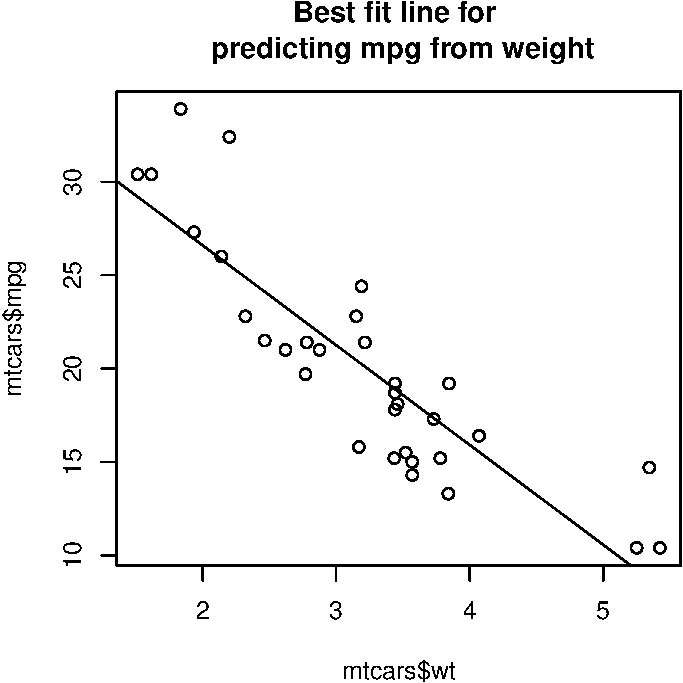
\includegraphics{visualisering_22_files/figure-latex/unnamed-chunk-45-1.pdf}

Man skriver relationen i R som \texttt{mpg\ \textasciitilde{}\ wt} og benytter \texttt{lm()}(\texttt{lm(mpg\textasciitilde{}wt,data=mtcars)}):

\begin{Shaded}
\begin{Highlighting}[]
\NormalTok{mylm }\OtherTok{\textless{}{-}} \FunctionTok{lm}\NormalTok{(mpg }\SpecialCharTok{\textasciitilde{}}\NormalTok{ wt, }\AttributeTok{data=}\NormalTok{mtcars)  }\CommentTok{\# build linear regression model}
\NormalTok{mylm}
\end{Highlighting}
\end{Shaded}

\begin{verbatim}
## 
## Call:
## lm(formula = mpg ~ wt, data = mtcars)
## 
## Coefficients:
## (Intercept)           wt  
##      37.285       -5.344
\end{verbatim}

Vores ``Coefficients'' beskriver den bedste rette linje:

\begin{itemize}
\tightlist
\item
  Skæringen (intercept): 37.285
\item
  Hældningskoefficient (slope): -5.344
\end{itemize}

Det betyder, at hvis vægten \texttt{wt} af en bil stiger med 1, så stiger \texttt{mpg} ved -5.344 (det vil sige at \texttt{mpg} reduceres med 5.344).

\hypertarget{r-squared-coefficient-of-determination}{%
\subsection{R-squared coefficient of determination}\label{r-squared-coefficient-of-determination}}

Den \(R^2\) eller ``forklaringsgraden'' (coefficeint of determination) har til formål at forklare, hvor godt vores lineær model passer til de data. For eksempel hvor meget af variansen i \texttt{mpg} forklares af variablen \texttt{wt}?

\begin{itemize}
\tightlist
\item
  Hvis det er tæt på 1 - så er der en meget tæt relation (hvis man kender vægten, så vide man også \texttt{mpg} med stor sikkerhed)
\item
  Hvis det er tæt på 0 - så er relationen svag - høj sandsynlighed for, at der er andre variabler der bedre kan forklare variansen i \texttt{mpg}.
\end{itemize}

I ovenstående model, kan man se den \(R^2\) værdi med \texttt{summary(mylm)}.

\begin{Shaded}
\begin{Highlighting}[]
\FunctionTok{summary}\NormalTok{(mylm)}
\end{Highlighting}
\end{Shaded}

\begin{verbatim}
## 
## Call:
## lm(formula = mpg ~ wt, data = mtcars)
## 
## Residuals:
##     Min      1Q  Median      3Q     Max 
## -4.5432 -2.3647 -0.1252  1.4096  6.8727 
## 
## Coefficients:
##             Estimate Std. Error t value Pr(>|t|)    
## (Intercept)  37.2851     1.8776  19.858  < 2e-16 ***
## wt           -5.3445     0.5591  -9.559 1.29e-10 ***
## ---
## Signif. codes:  0 '***' 0.001 '**' 0.01 '*' 0.05 '.' 0.1 ' ' 1
## 
## Residual standard error: 3.046 on 30 degrees of freedom
## Multiple R-squared:  0.7528, Adjusted R-squared:  0.7446 
## F-statistic: 91.38 on 1 and 30 DF,  p-value: 1.294e-10
\end{verbatim}

Det fortæller os, at \(R^2\) = 0.7528.

\hypertarget{antagelser---lineuxe6r-regression}{%
\subsection{Antagelser - lineær regression}\label{antagelser---lineuxe6r-regression}}

\begin{itemize}
\tightlist
\item
  Normalfordelte residualer
\item
  Residualer har samme spredning (varianshomogenitet)
\item
  Uafhængighed
\item
  Fit er linæer
\end{itemize}

Koden \texttt{plot(mylm,which=c(1))} angiver residualer vs predikterede (fitted) værdier - de skal være tilfældigt fordelt over plottet og prikkernes varians skal være nogenlunde konstant langt x-aksen (det giver, at den røde linje er flade).

\begin{Shaded}
\begin{Highlighting}[]
\FunctionTok{plot}\NormalTok{(mylm,}\AttributeTok{which=}\FunctionTok{c}\NormalTok{(}\DecValTok{1}\NormalTok{))}
\end{Highlighting}
\end{Shaded}

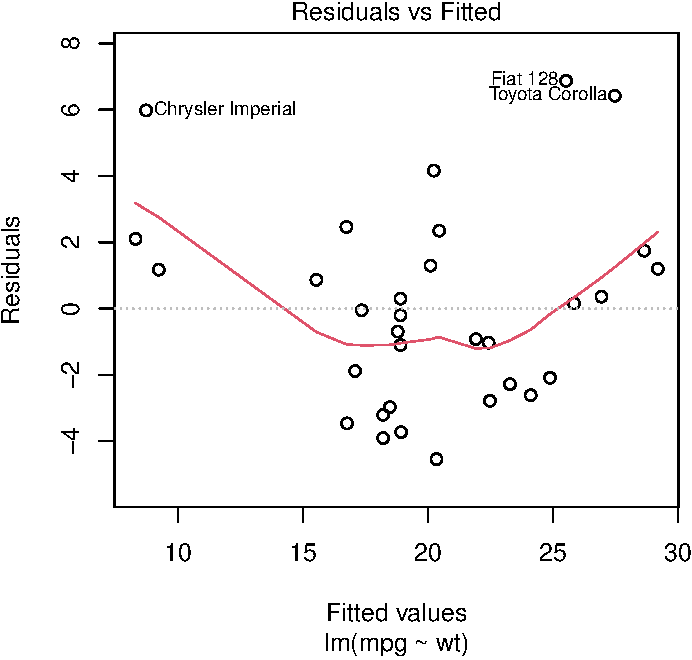
\includegraphics{visualisering_22_files/figure-latex/unnamed-chunk-48-1.pdf}

Med koden \texttt{plot(mylm,which=c(2))} kan man tjekke antagelsen på en normal fordeling. Punkterne skal være nogenlunde tæt på den diagonale linje.

\begin{Shaded}
\begin{Highlighting}[]
\FunctionTok{plot}\NormalTok{(mylm,}\AttributeTok{which=}\FunctionTok{c}\NormalTok{(}\DecValTok{2}\NormalTok{))}
\end{Highlighting}
\end{Shaded}

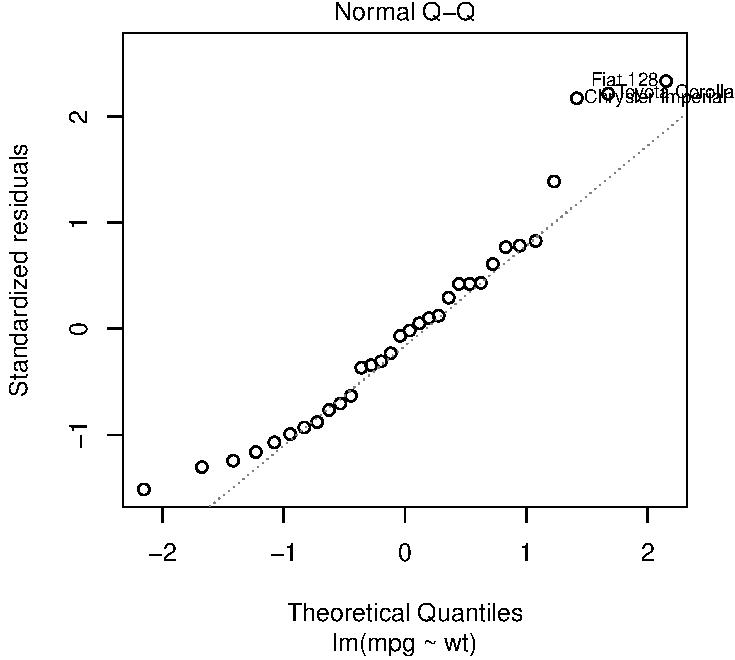
\includegraphics{visualisering_22_files/figure-latex/unnamed-chunk-49-1.pdf}

\hypertarget{multiple-lineuxe6r-regression}{%
\subsection{Multiple lineær regression}\label{multiple-lineuxe6r-regression}}

Her kan man tilføje flere variabler i vores model formel.

\begin{Shaded}
\begin{Highlighting}[]
\NormalTok{mylm\_disp }\OtherTok{\textless{}{-}} \FunctionTok{lm}\NormalTok{(mpg }\SpecialCharTok{\textasciitilde{}}\NormalTok{ wt }\SpecialCharTok{+}\NormalTok{ disp, }\AttributeTok{data=}\NormalTok{mtcars) }\CommentTok{\# build linear regression model}
\FunctionTok{summary}\NormalTok{(mylm\_disp)}
\end{Highlighting}
\end{Shaded}

\begin{verbatim}
## 
## Call:
## lm(formula = mpg ~ wt + disp, data = mtcars)
## 
## Residuals:
##     Min      1Q  Median      3Q     Max 
## -3.4087 -2.3243 -0.7683  1.7721  6.3484 
## 
## Coefficients:
##             Estimate Std. Error t value Pr(>|t|)    
## (Intercept) 34.96055    2.16454  16.151 4.91e-16 ***
## wt          -3.35082    1.16413  -2.878  0.00743 ** 
## disp        -0.01773    0.00919  -1.929  0.06362 .  
## ---
## Signif. codes:  0 '***' 0.001 '**' 0.01 '*' 0.05 '.' 0.1 ' ' 1
## 
## Residual standard error: 2.917 on 29 degrees of freedom
## Multiple R-squared:  0.7809, Adjusted R-squared:  0.7658 
## F-statistic: 51.69 on 2 and 29 DF,  p-value: 2.744e-10
\end{verbatim}

Her kan man se, at med tilføjelsen af variablen \texttt{disp}, er \(R^2\) steget til 0.7809. Bemærk, at jo flere variabler man tilføjer til modellen, jo større bliver \(R^2\)-værdien. Den adjusted \(R^2\) værdi er lavere fordi den prøver at tage højde for kompleksiteten af modellen (hvor mange parametre der er).

Variablen \texttt{disp} er faktisk ikke selv signifikant når der er taget højde for variablen \texttt{wt} (p-værdien 0.0636 - tjek, at du selv kan finde værdien i resultatet).

Hvis en af de uafhængige variabler er kategorisk bruger man funktionen \texttt{anova} til at teste den overordnet effekt af den variabel. For eksempel har variablen \texttt{cyl} 3 mulige værdier (niveauer) - 4, 6 og 8. Vi kan inddrage variablen i vores model: --\textgreater{}

\begin{Shaded}
\begin{Highlighting}[]
\NormalTok{mylm\_cyl }\OtherTok{\textless{}{-}} \FunctionTok{lm}\NormalTok{(mpg }\SpecialCharTok{\textasciitilde{}}\NormalTok{ wt }\SpecialCharTok{+} \FunctionTok{factor}\NormalTok{(cyl), }\AttributeTok{data=}\NormalTok{mtcars) }\CommentTok{\# build linear regression model}
\FunctionTok{summary}\NormalTok{(mylm\_cyl)}
\end{Highlighting}
\end{Shaded}

\begin{verbatim}
## 
## Call:
## lm(formula = mpg ~ wt + factor(cyl), data = mtcars)
## 
## Residuals:
##     Min      1Q  Median      3Q     Max 
## -4.5890 -1.2357 -0.5159  1.3845  5.7915 
## 
## Coefficients:
##              Estimate Std. Error t value Pr(>|t|)    
## (Intercept)   33.9908     1.8878  18.006  < 2e-16 ***
## wt            -3.2056     0.7539  -4.252 0.000213 ***
## factor(cyl)6  -4.2556     1.3861  -3.070 0.004718 ** 
## factor(cyl)8  -6.0709     1.6523  -3.674 0.000999 ***
## ---
## Signif. codes:  0 '***' 0.001 '**' 0.01 '*' 0.05 '.' 0.1 ' ' 1
## 
## Residual standard error: 2.557 on 28 degrees of freedom
## Multiple R-squared:  0.8374, Adjusted R-squared:   0.82 
## F-statistic: 48.08 on 3 and 28 DF,  p-value: 3.594e-11
\end{verbatim}

Man kan ikke se den overordnet effekt af \texttt{cyl} fra den ovenstående \texttt{summary} men man kan teste den med \texttt{anova}:

\begin{Shaded}
\begin{Highlighting}[]
\FunctionTok{anova}\NormalTok{(mylm,mylm\_cyl)}
\end{Highlighting}
\end{Shaded}

\begin{verbatim}
## Analysis of Variance Table
## 
## Model 1: mpg ~ wt
## Model 2: mpg ~ wt + factor(cyl)
##   Res.Df    RSS Df Sum of Sq      F   Pr(>F)   
## 1     30 278.32                                
## 2     28 183.06  2    95.263 7.2856 0.002835 **
## ---
## Signif. codes:  0 '***' 0.001 '**' 0.01 '*' 0.05 '.' 0.1 ' ' 1
\end{verbatim}

Så kan man se, at \texttt{cyl} er signifikant.

\hypertarget{problemstillinger}{%
\section{Problemstillinger}\label{problemstillinger}}

Alle bør lave quizzen men ellers vælg øvelser efter egen erfaring:

\begin{itemize}
\tightlist
\item
  2-7 er meget grundlæggende og de fleste kan springer over hvis nogenlunde tryg med base-R
\item
  8-14 anbefaler jeg til alle som en god måde at tjekke viden på
\item
  15-18 øver hvordan man laver variansanalyse/regression i R - regression kommer jeg ind på igen senere men det hjælper hvis du er tryg med brugen af funktionen \texttt{lm} til at lave modeller i ANOVA/simpel lineær regression.
\end{itemize}

\hypertarget{quiz---basics}{%
\subsection{Quiz - Basics}\label{quiz---basics}}

\begin{enumerate}
\def\labelenumi{\arabic{enumi})}
\tightlist
\item
  Se quiz i Absalon, der hedder ``Quiz - Basics''.
\end{enumerate}

\hypertarget{grundluxe6ggende-r}{%
\subsection{Grundlæggende R}\label{grundluxe6ggende-r}}

\begin{enumerate}
\def\labelenumi{\arabic{enumi})}
\setcounter{enumi}{1}
\tightlist
\item
  (\textbf{helt baserende viden}) Åbn en ny fil i Rstudio ved at trykke på ``File'' \textgreater{} ``New File'' \textgreater{} ``R script''. Køre følgende kode en linje ad gangen og tjek, du kan forstå outputtet.
\end{enumerate}

Husk at den nemmeste måde at køre kode er ved at trykke CMD+ENTER (Mac) eller WIN-KEY+ENTER (Windows).

\begin{Shaded}
\begin{Highlighting}[]
\DecValTok{2}\SpecialCharTok{+}\DecValTok{2}
\DecValTok{2}\SpecialCharTok{*}\DecValTok{2}
\NormalTok{x }\OtherTok{\textless{}{-}} \DecValTok{4}
\NormalTok{x }\OtherTok{\textless{}{-}}\NormalTok{ x}\SpecialCharTok{+}\DecValTok{2}
\FunctionTok{sqrt}\NormalTok{(x)}
\FunctionTok{sqrt}\NormalTok{(x)}\SpecialCharTok{\^{}}\DecValTok{2}
\FunctionTok{rnorm}\NormalTok{(}\DecValTok{10}\NormalTok{,}\DecValTok{2}\NormalTok{,}\DecValTok{2}\NormalTok{)}
\FunctionTok{log10}\NormalTok{(}\DecValTok{100}\NormalTok{)}
\NormalTok{y }\OtherTok{\textless{}{-}}  \FunctionTok{c}\NormalTok{(}\DecValTok{1}\NormalTok{,}\DecValTok{4}\NormalTok{,}\DecValTok{6}\NormalTok{,}\DecValTok{4}\NormalTok{,}\DecValTok{3}\NormalTok{)}
\FunctionTok{class}\NormalTok{(y)}
\FunctionTok{class}\NormalTok{(}\FunctionTok{c}\NormalTok{(}\StringTok{"a"}\NormalTok{,}\StringTok{"b"}\NormalTok{,}\StringTok{"c"}\NormalTok{))}
\FunctionTok{mean}\NormalTok{(y)}
\FunctionTok{sd}\NormalTok{(y)}
\FunctionTok{seq}\NormalTok{(}\DecValTok{1}\NormalTok{,}\DecValTok{13}\NormalTok{,}\AttributeTok{by=}\DecValTok{3}\NormalTok{)}
\end{Highlighting}
\end{Shaded}

\begin{enumerate}
\def\labelenumi{\arabic{enumi})}
\setcounter{enumi}{2}
\tightlist
\item
  (\textbf{helt baserende viden}) Køre følgende kode til at åbne nogle af de indbygget datasæt, som vi bruger i kurset.
\end{enumerate}

\begin{itemize}
\tightlist
\item
  Prøve \texttt{head()}, \texttt{nrow()}, \texttt{summary()} osv.
\item
  Prøve også fk. \texttt{?cars} for at se en beskrivelse.
\end{itemize}

\begin{Shaded}
\begin{Highlighting}[]
\FunctionTok{data}\NormalTok{(iris)}
\FunctionTok{data}\NormalTok{(cars)}
\FunctionTok{data}\NormalTok{(ToothGrowth)}
\FunctionTok{data}\NormalTok{(sleep)}
\FunctionTok{head}\NormalTok{(chickwts)}
\FunctionTok{data}\NormalTok{(trees)}
\CommentTok{\#se her for andre:}
\FunctionTok{library}\NormalTok{(}\AttributeTok{help =} \StringTok{"datasets"}\NormalTok{)}
\end{Highlighting}
\end{Shaded}

\begin{enumerate}
\def\labelenumi{\arabic{enumi})}
\setcounter{enumi}{3}
\tightlist
\item
  (\textbf{baserende plots}) Jeg giver nogle muligheder for datasættet ``iris''. Afprøve funktionerne for nogle af de andre ovenstående indbygget datasæt, som du indlæst.
\end{enumerate}

\begin{Shaded}
\begin{Highlighting}[]
\FunctionTok{plot}\NormalTok{(iris}\SpecialCharTok{$}\NormalTok{Sepal.Length,iris}\SpecialCharTok{$}\NormalTok{Sepal.Width)}
\FunctionTok{hist}\NormalTok{(iris}\SpecialCharTok{$}\NormalTok{Sepal.Width)}
\FunctionTok{boxplot}\NormalTok{(iris}\SpecialCharTok{$}\NormalTok{Sepal.Length}\SpecialCharTok{\textasciitilde{}}\NormalTok{iris}\SpecialCharTok{$}\NormalTok{Species)}
\end{Highlighting}
\end{Shaded}

Man kan også gøre plotterne lidt pænere ved at give dem en titel/aksen-navne osv. Prøve \texttt{?plot} for at se nogle muligheder, og tilføje \texttt{ylab}, \texttt{xlab}, \texttt{main} (titel) i én af plotterne. Leg også med \texttt{col} (farver). Bemærk dog, at vi kommer til at ændre måden at lave plotter på når vi starter \texttt{ggplot2}.

\begin{enumerate}
\def\labelenumi{\arabic{enumi})}
\setcounter{enumi}{4}
\tightlist
\item
  (\textbf{dataframes}) Brug datasættet \texttt{cars} (\texttt{data(cars)}) til at:
\end{enumerate}

\begin{itemize}
\tightlist
\item
  Lav et scatter plot med speed på x-aksen og dist på y-aksen
\item
  Tilføj en ny kolon med følgende kode:
\end{itemize}

\begin{Shaded}
\begin{Highlighting}[]
\NormalTok{cars}\SpecialCharTok{$}\NormalTok{fast }\OtherTok{\textless{}{-}}\NormalTok{ cars}\SpecialCharTok{$}\NormalTok{speed}\SpecialCharTok{\textgreater{}}\DecValTok{15}
\end{Highlighting}
\end{Shaded}

\begin{itemize}
\tightlist
\item
  Brug \texttt{mean} på den nye variabel til at finde ud af proportionen af biler, der er hurtige
\item
  Beregn gennemsnitsværdien af variablen \texttt{dist} for hurtige biler og ikke-hurtige biler hver for sig (brug funktionen \texttt{tapply}). Gem resultatet med \texttt{\textless{}-}.
\item
  Brug \texttt{barplot} til at lave et plot af den gennemsnitlige \texttt{dist} for hurtige og ikke-hurtige biler.
\end{itemize}

\begin{enumerate}
\def\labelenumi{\arabic{enumi})}
\setcounter{enumi}{4}
\tightlist
\item
  (\textbf{dataframes}) Lav en ny dataframe (funktionen \texttt{data.frame()}) med tre kolonner som hedder ``navn'', ``alder'' og ``yndlings\_farve'' (find bare selv på værdierne). Sørge for, at den har 4 rækker.
\end{enumerate}

\begin{Shaded}
\begin{Highlighting}[]
\NormalTok{mydf }\OtherTok{\textless{}{-}} \FunctionTok{data.frame}\NormalTok{(}\StringTok{"navn"}\OtherTok{=} \FunctionTok{c}\NormalTok{(}\StringTok{"alice"}\NormalTok{,}\StringTok{"freddy"}\NormalTok{, ... ), }\StringTok{"alder"} \OtherTok{=} \FunctionTok{c}\NormalTok{(...), ...) }\CommentTok{\#not run, slette "..." og skrive videre}
\FunctionTok{dim}\NormalTok{(mydf) }\CommentTok{\# fire række og tre kolonner}
\NormalTok{mydf}
\end{Highlighting}
\end{Shaded}

\begin{enumerate}
\def\labelenumi{\arabic{enumi})}
\setcounter{enumi}{5}
\tightlist
\item
  (\textbf{dataframes}) Tilføj en ny variabel \texttt{random} til ovenstående dataframe, hvor værdierne kommer fra en normal fordeling med et gennemsnit på 5 og sd på 1 (bruge funktionen \texttt{rnorm}).
\end{enumerate}

\begin{Shaded}
\begin{Highlighting}[]
\NormalTok{mydf}\SpecialCharTok{$}\NormalTok{random }\OtherTok{\textless{}{-}} \CommentTok{\#??}
\end{Highlighting}
\end{Shaded}

\begin{enumerate}
\def\labelenumi{\arabic{enumi})}
\setcounter{enumi}{6}
\tightlist
\item
  (\textbf{delmængder af dataframes}) Åbn datasættet ``ToothGrowth'' med følgende kode:
\end{enumerate}

\begin{Shaded}
\begin{Highlighting}[]
\FunctionTok{data}\NormalTok{(}\StringTok{"ToothGrowth"}\NormalTok{)}
\NormalTok{?ToothGrowth}
\end{Highlighting}
\end{Shaded}

\begin{itemize}
\tightlist
\item
  Find delmængden af datasættet således at diet (variablen \texttt{supp}) er ``OJ'' og længden (variablen \texttt{len}) er større end 15.
\end{itemize}

\begin{Shaded}
\begin{Highlighting}[]
\NormalTok{newdf }\OtherTok{\textless{}{-}}\NormalTok{ ToothGrowth[}\CommentTok{\#skrive her til at lave subset af observationerne,]}
\end{Highlighting}
\end{Shaded}

\begin{itemize}
\tightlist
\item
  Hvor mange rækker er der i den nye dataframe \texttt{newdf}?
\item
  Hvor mange unikke værdier er der i variablen \texttt{dose} (brug funktionen \texttt{unique}) ?
\item
  Find delmængden af datasættet \texttt{ToothGrowth}, hvor variablen \texttt{dose} er 0.5 eller 1.5 (hint: brug \texttt{\%in\%} eller \texttt{\textbar{}}) og \texttt{supp} er ``VC''.
\item
  Beregn den gennemsnitlige længde for observationerne i delmængden.
\end{itemize}

\hypertarget{kort-analyse-med-reaktionstider}{%
\subsection{Kort analyse med reaktionstider}\label{kort-analyse-med-reaktionstider}}

\begin{enumerate}
\def\labelenumi{\arabic{enumi})}
\setcounter{enumi}{7}
\tightlist
\item
  (\textbf{indlæse data}) Åbn en fil, der sidder i Absalon og hedder ``reactions.txt'' ved at bruge funktionen \texttt{read.table()} (giv objektet et navn, e.g.~\texttt{data}). Husk at tjekke, om filen har en `header' og bruge således \texttt{header=T} hvis nødvendigt.
\end{enumerate}

\begin{Shaded}
\begin{Highlighting}[]
\NormalTok{data }\OtherTok{\textless{}{-}}\NormalTok{ ... }\CommentTok{\#replace ...}
\end{Highlighting}
\end{Shaded}

\begin{enumerate}
\def\labelenumi{\arabic{enumi})}
\setcounter{enumi}{8}
\tightlist
\item
  (\textbf{factor variabler}) Variablerne \texttt{subject} og \texttt{time} indlæses som henholdvis data type `int' (heltal) og ``chr'' (character) men de skal hellere være `factor' variabler. Lav dem om til facktor variabler, fk.
\end{enumerate}

\begin{Shaded}
\begin{Highlighting}[]
\NormalTok{data}\SpecialCharTok{$}\NormalTok{subject }\OtherTok{\textless{}{-}} \FunctionTok{as.factor}\NormalTok{(data}\SpecialCharTok{$}\NormalTok{subject) }\CommentTok{\#gør subject til en faktor}
\DocumentationTok{\#\# gør den samme her for time:}
\NormalTok{data}\SpecialCharTok{$}\NormalTok{...}
\end{Highlighting}
\end{Shaded}

\begin{enumerate}
\def\labelenumi{\arabic{enumi})}
\setcounter{enumi}{9}
\tightlist
\item
  (\textbf{delmængde af dataframe})
\end{enumerate}

Lav to delmængder af ovenstående datasæt -

\begin{itemize}
\tightlist
\item
  én til alle observationer fra tidspunktet ``before'' (\texttt{time\ =="before"}) og
\item
  én til alle observationer fra tidspunktet ``after''.
\end{itemize}

\begin{Shaded}
\begin{Highlighting}[]
\NormalTok{RT\_before }\OtherTok{\textless{}{-}}\NormalTok{ data[}\CommentTok{\#skrive her , ]}
\NormalTok{RT\_after }\OtherTok{\textless{}{-}} \CommentTok{\#skrive her}
\end{Highlighting}
\end{Shaded}

\begin{enumerate}
\def\labelenumi{\arabic{enumi})}
\setcounter{enumi}{10}
\tightlist
\item
  (\textbf{mean og tapply}) Benyt funktionen \texttt{mean} til at beregne den gennemsnitlige reaktionstid (variablen \texttt{RT}) til ``before'' og ``after'' hver for sig (brug ovenstående delmængder).
\end{enumerate}

\begin{itemize}
\tightlist
\item
  Prøv også at anvende funktionen \texttt{tapply} på det oprindelige datasæt til at gøre den samme med mindre kode.
\end{itemize}

\begin{Shaded}
\begin{Highlighting}[]
\FunctionTok{tapply}\NormalTok{(}\CommentTok{\#skrive her,\#skrive her,\#skrive her)}
\end{Highlighting}
\end{Shaded}

\begin{enumerate}
\def\labelenumi{\arabic{enumi})}
\setcounter{enumi}{11}
\tightlist
\item
  (\textbf{beregn forskellen og mean})
\end{enumerate}

Bemærk datasættet er `paired' - målingerne er lavet på de samme personer både ``before'' og ``after''. --\textgreater{}

\begin{itemize}
\tightlist
\item
  Lav en vector \texttt{diff}, der er ændringen i reaktionstiderne mellem ``before'' og ``after''.
\item
  Beregn den gennemsnitlige forskel i rekationstiderne over de 10 personer.
\end{itemize}

\begin{Shaded}
\begin{Highlighting}[]
\NormalTok{diff }\OtherTok{\textless{}{-}} \CommentTok{\#change in reaction time between before and after}
\FunctionTok{mean}\NormalTok{(diff)}
\end{Highlighting}
\end{Shaded}

\begin{enumerate}
\def\labelenumi{\arabic{enumi})}
\setcounter{enumi}{12}
\tightlist
\item
  (\textbf{lav t-test i R}) Lav en t-test (funktionen \texttt{t.test}) for at teste hypotesen at ændringen i reaktionstiderne mellem ``before'' og ``after'' er anderledes end 0.
\end{enumerate}

\begin{Shaded}
\begin{Highlighting}[]
\FunctionTok{t.test}\NormalTok{(}\CommentTok{\#skrive her..)}
\end{Highlighting}
\end{Shaded}

Find følgende i outputtet fra R:

\begin{itemize}
\tightlist
\item
  Hvor er test-statistikken \texttt{t}?
\item
  Hvor er p-værdien?
\item
  Hvad er alternativhypotesen?
\end{itemize}

\begin{enumerate}
\def\labelenumi{\arabic{enumi})}
\setcounter{enumi}{13}
\tightlist
\item
  Skriv en kort sætning med din konklusion.
\end{enumerate}

\hypertarget{uxf8velser-med-statistik-tests}{%
\subsection{Øvelser med statistik tests}\label{uxf8velser-med-statistik-tests}}

\begin{enumerate}
\def\labelenumi{\arabic{enumi})}
\setcounter{enumi}{14}
\tightlist
\item
  (\textbf{Chi-sq}) Kør følgende kode til at få en tabel (selve koden er ikke vigtigt):
\end{enumerate}

\begin{Shaded}
\begin{Highlighting}[]
\NormalTok{mytable }\OtherTok{\textless{}{-}} \FunctionTok{structure}\NormalTok{(}\FunctionTok{c}\NormalTok{(80L, 97L, 372L, 136L, 87L, 119L), }\AttributeTok{.Dim =} \DecValTok{3}\SpecialCharTok{:}\DecValTok{2}\NormalTok{, }\AttributeTok{.Dimnames =} \FunctionTok{structure}\NormalTok{(}\FunctionTok{list}\NormalTok{(}
    \FunctionTok{c}\NormalTok{(}\StringTok{"First"}\NormalTok{, }\StringTok{"Second"}\NormalTok{, }\StringTok{"Third"}\NormalTok{), }\FunctionTok{c}\NormalTok{(}\StringTok{"Died"}\NormalTok{, }\StringTok{"Survived"}\NormalTok{)), }\AttributeTok{.Names =} \FunctionTok{c}\NormalTok{(}\StringTok{"Class"}\NormalTok{, }\StringTok{"Survival"}\NormalTok{)), }\AttributeTok{class =} \StringTok{"table"}\NormalTok{)}

\NormalTok{mytable}
\end{Highlighting}
\end{Shaded}

\begin{verbatim}
##         Survival
## Class    Died Survived
##   First    80      136
##   Second   97       87
##   Third   372      119
\end{verbatim}

Tabellen omhandler personer ombord skibet `Titanic' - den angiver hvor mange passagerer tilhørte de tre klass (førsteklass, andenklass, trejdeklass), delte efter overlevelse (døde eller overlevede tragedien).

\begin{itemize}
\tightlist
\item
  Benyt funktionen \texttt{chisq.test()} på tabellen.
\item
  Hvad er nulhypotesen?
\item
  Er testen signifikant?
\item
  Er passagerernes klass så uafhængige af deres chance for at overleve tragedien?
\item
  Hvilken klass havde den bedste chance for at overleve?
\end{itemize}

\begin{enumerate}
\def\labelenumi{\arabic{enumi})}
\setcounter{enumi}{16}
\tightlist
\item
  (\textbf{Korrelation analyse}) Åbn datasættet \texttt{trees} og lav et scatter plot med variablen \texttt{Girth} på x-aksen og variablen \texttt{Volume} på y-aksen.
\end{enumerate}

\begin{Shaded}
\begin{Highlighting}[]
\FunctionTok{data}\NormalTok{(trees)}
\FunctionTok{summary}\NormalTok{(trees)}
\end{Highlighting}
\end{Shaded}

\begin{itemize}
\tightlist
\item
  Anvend funktionen \texttt{cor.test} for at teste, om der er en signifikant korrelation mellem de to variabler. Brug \texttt{method\ =\ "pearson"} (det er dog faktisk default)
\end{itemize}

\begin{Shaded}
\begin{Highlighting}[]
\FunctionTok{cor.test}\NormalTok{(???, ???,}\AttributeTok{method=}\StringTok{"pearson"}\NormalTok{)}
\end{Highlighting}
\end{Shaded}

\begin{itemize}
\tightlist
\item
  Hvad er korrelationen mellem \texttt{Girth} og \texttt{Volume}?
\item
  Hvad er p-værdien? Er den signifikant?
\end{itemize}

\begin{enumerate}
\def\labelenumi{\arabic{enumi})}
\setcounter{enumi}{14}
\tightlist
\item
  (\textbf{ANOVA}) OBS: hvis du føler dig utryg med funktionen \texttt{lm()} - der kommer en video om det i morgen (i forbindelse med emnet Rmarkdown).
\end{enumerate}

Kør følgende kode til at lave variansanalyse, der tester hulhypotesen hvor den gennemsnitlige værdi af variablen \texttt{Sepal.Width} er ens for hver af de tre arter (variablen \texttt{Species}) fra datasættet \texttt{iris}:

\begin{Shaded}
\begin{Highlighting}[]
\FunctionTok{data}\NormalTok{(iris)}

\CommentTok{\#model under H0: no difference according to Species (1 just means "fit overall mean")}
\NormalTok{model\_h0 }\OtherTok{\textless{}{-}} \FunctionTok{lm}\NormalTok{(Sepal.Width }\SpecialCharTok{\textasciitilde{}} \DecValTok{1}\NormalTok{, }\AttributeTok{data=}\NormalTok{iris) }

\CommentTok{\#model under H1: each level of Species has its own mean}
\NormalTok{model\_h1 }\OtherTok{\textless{}{-}} \FunctionTok{lm}\NormalTok{(Sepal.Width }\SpecialCharTok{\textasciitilde{}}\NormalTok{ Species, }\AttributeTok{data=}\NormalTok{iris) }

\CommentTok{\#compare two models {-} significant p{-}value equates to choosing H1 model}
\FunctionTok{anova}\NormalTok{(model\_h0,model\_h1)}
\end{Highlighting}
\end{Shaded}

Kig på outputtet:

\begin{itemize}
\tightlist
\item
  Hvilken model reflekterer nulhypotesen?
\item
  Hvilken model reflekterer alternativhypotesen?
\item
  Hvor er p-værdien?
\item
  Er der en signifikant forskel i den gennemsnitlige \texttt{Sepal.Width} efter de forskellige \texttt{Species}?
\end{itemize}

Brug funktionen \texttt{tapply} for at finde ud af, hvad er den middelværdi \texttt{Sepal.Width} til hver af de tre arter.

\begin{enumerate}
\def\labelenumi{\arabic{enumi})}
\setcounter{enumi}{15}
\tightlist
\item
  (\textbf{ANOVA}) Lav en lignende analyse på datasættet \texttt{chickwts} for at svare på spørgsmålet:
\end{enumerate}

\begin{itemize}
\tightlist
\item
  Er der en forskel i den gennemsnitlige vægt (variablen \texttt{weight}) efter fodertypen (variablen \texttt{feed})? Med andre ord er vægt afhængig af fodertypen?
\end{itemize}

\begin{Shaded}
\begin{Highlighting}[]
\FunctionTok{data}\NormalTok{(chickwts)}
\CommentTok{\#skriv kode herfra}
\end{Highlighting}
\end{Shaded}

\begin{enumerate}
\def\labelenumi{\arabic{enumi})}
\setcounter{enumi}{17}
\tightlist
\item
  (\textbf{Lineær regression})
\end{enumerate}

\begin{itemize}
\tightlist
\item
  Brug \texttt{lm} til at lave en simpel lineær regression, således at respons variablen \texttt{Volume} er afhængig af variablen \texttt{Girth} (datasæstet \texttt{trees}).
\end{itemize}

\begin{Shaded}
\begin{Highlighting}[]
\NormalTok{mylm }\OtherTok{\textless{}{-}} \FunctionTok{lm}\NormalTok{(???, }\AttributeTok{data=}\NormalTok{trees) }
\end{Highlighting}
\end{Shaded}

Brug \texttt{summary} på din model for at finde følgende værdier:

\begin{itemize}
\tightlist
\item
  Hvad er r.squared? (multiple)
\item
  Er variablen \texttt{Girth} signifikant?
\item
  Hvad er ligningen på den bedste rette linje (husk formen y = ax + b)?
\end{itemize}

\begin{enumerate}
\def\labelenumi{\arabic{enumi})}
\setcounter{enumi}{17}
\tightlist
\item
  (\textbf{Kort intro til multiple lineær regression}) Tag ovenstående model og tilføj variablen \texttt{Height} som en ekstra prediktær (uafhængig) variabel i modellen med en ``+'' tegn:
\end{enumerate}

\begin{Shaded}
\begin{Highlighting}[]
\NormalTok{mylm\_height }\OtherTok{\textless{}{-}} \FunctionTok{lm}\NormalTok{(??? }\SpecialCharTok{\textasciitilde{}}\NormalTok{ ??? }\SpecialCharTok{+}\NormalTok{ ???, }\AttributeTok{data=}\NormalTok{trees) }
\FunctionTok{summary}\NormalTok{(mylm\_height)}
\end{Highlighting}
\end{Shaded}

\emph{Bemærk at det ikke betyder, at de to variabler skal lægges sammen, men at vi gerne vil have både variablerne i modellen som uafhængig variabler (med andre ord er \texttt{Volume} afhængig af både \texttt{Girth} og \texttt{Height}).}

Benyt \texttt{summary} på modellen og prøv at finde følgende:

\begin{itemize}
\tightlist
\item
  Hvad er den den (multiple) r.squared værdi?
\item
  Hvor meget ændre den (multiple) r.squared værdi i forhold til modellen med kun variablen \texttt{Girth}?
\item
  Er \texttt{Volume} signifikant afhængig af \texttt{Height} (efter at man har taget højde for \texttt{Girth})?
\end{itemize}

Brug funktionen \texttt{anova} til at sammenligne modellen uden \texttt{Height} med modellen med \texttt{Height}

\begin{Shaded}
\begin{Highlighting}[]
\FunctionTok{anova}\NormalTok{(}\CommentTok{\#model without height,\#model with height)}
\end{Highlighting}
\end{Shaded}

Bemærk, at i dette tilfælde er p-værdien fra ANOVA samme p-værdi fra \texttt{summary(mylm\_height)}.

  \bibliography{book.bib,packages.bib}

\end{document}
